\section{实验:测滑轮组的机械效率}\label{sec:8-6}

\begin{wrapfigure}[16]{r}{6cm}
    \centering
    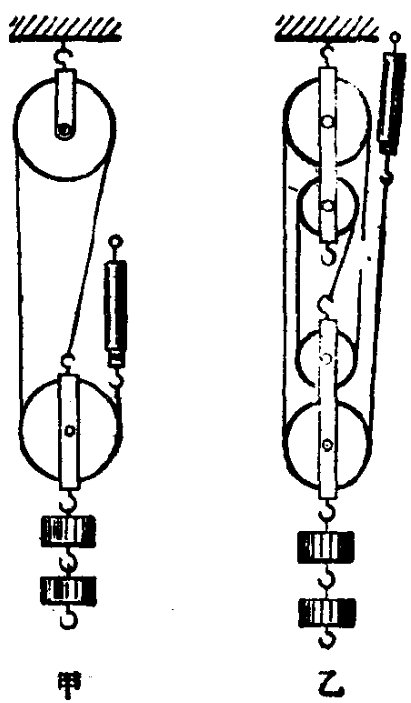
\includegraphics[width=5cm]{../pic/czwl1-ch8-9}
    \caption{}\label{fig:8-9}
\end{wrapfigure}

\shiyan{目的} 测滑轮组的机械效率。

\shiyan{器材} 刻度尺,弹簧秤,钩码,铁架台,一个定滑轮和一个动滑轮组成的滑轮组,
两个定滑轮和两个动滑轮组成的滑轮组,长约 2 米的细绳。

\shiyan{步驟}

(1) 照图 \ref{fig:8-9} 甲那样,把实验装置安装好。细绳的一端先拴在动滑轮上,然后顺次穿过定滑轮、动滑轮,
另一端拴在弹簧秤上。在动滑轮下面挂上钩码,并分别记下钩码和弹簧秤的位置。

(2) 向上拉弹簧秤,使钩码匀速上升一段距离。从弹簧秤上读出拉力的大小。
用刻度尺分别量出钩码和弹簧秤移动的距离。

(3) 算出总功、有用功。这个滑轮组的机械效率是多少?

(4) 再照图 \ref{fig:8-9} 乙那样换用由两个定滑轮和两个动滑轮组成的滑轮组来做实验,
算出总功、有用功和滑轮组的机械效率。为什么这个滑轮组的机械效率比甲图的低?

根据上述实验步骤,设计一张表格,将有关数据填入表中。


\lianxi

(1) 沿着长 5 米、高 1 米的斜面,把重 $10^4$ 牛顿的物体拉到车上去,做的有用功是多少?
如果所用的拉力是 2500 牛顿,做的总功是多少?这个斜面的机械效率是多少?

(2) 用图 \ref{fig:7-27} 所示的滑轮组提起重 2000 牛顿的货物,所用的拉力是 800 牛顿,
绳子的自由端被拉下了 4 米,我们对滑轮组做的总功是多少?滑轮组提起货物做的有用功是多少?
这个滑轮组的机械效率是多少?

(3) 用滑轮组把 720 牛顿的货物提高 10 米,滑轮组的机械效率是 $60\%$,求做的总功。

